\chapter{Approach}

Our approach aims to help software developers in remote teams who might be facing challenges with team awareness, informal communication within their team, and well-being. We aim to tackle these issues by allowing knowledge workers to easily learn about the availability, moods and emotions, and other states of their core team members. The key underlying concepts of our approach listed and explained in the following.

\medskip\noindent\textbf{General Design Decisions} \\
Overall, our approach follows a very social fundamental idea with the goal of reducing workplace isolation. To reduce the feeling of workplace isolation, our approach builds on the following two key design decisions.
\begin{enumerate}[itemsep=0ex, parsep=0ex, leftmargin=*]
    \item \textbf{Ambient and Minimal} \\
          At the core of our approach sits the desicion to create a tool that is ambient in nature and does not require significant, additional effort in order to be useful. Having a limited amount of information on an ambient display is critial for both not being interruptive and costly to use \autocite{dabbish2004controlling}. With the help of the ambient display, the goal is to create a sense of presence within the team. By constantly showing the most important team members the goal is to minimize the feeling of being left and to foster a sense of belonging.
    \item \textbf{People-centric} \\
          In comparison to existing awareness inceasing approaches with emphasis primarily on task related awareness and their implications for more effective and efficient collaboration, our approach puts the humans behind the work items into the center of focus. Individual moods and emotions play a fundamental role in our approach.
\end{enumerate}

\noindent With the large number of existing communication applications (e.g. eMail, Slack, Microsoft Teams, zoom.us, etc.) our goal is not to replace them in the first place but rather complement and enrich the content transmitted with otherwise hard to maintain information. This sought to be achieved by increasing workplace awareness and informal communication.
% \medskip\noindent\textbf{Customizability} \\
% "Teams in which membership is stable and long standing have been the target of traditional team research (Ancona, 1990; West and Lyubovnikova, 2012). However, nature of work in externally dependent teams in the areas of software development, new product development and coalitions demands flexible teams, which are capable of handling the complex nature of their work and dealing with a diverse external environment (Faraj and Yan, 2009). Software development teams are structured such that members work on **multiple teams simultaneously, and participate in projects at specific periods in the project life cycle as opposed to working on a single team throughout**. Some team members work on the core task of application development, while others may be associated with the team as business analysts, testers and as a part of quality assurance (Yang and Tang, 2004)." [dey2020impact](https://www.notion.so/dey2020impact-5ec814e274c64e439ef08107599318c5)

\medskip\noindent\textbf{Workplace awareness} \\
Being more aware of the core team members and their current availibility or emotional status, what they are working on, etc., several oportunities open to spontaneously interact with other teammembers while not interrupting them at in-opportune times.

\medskip\noindent\textbf{Informal communication} \\
The focus of this work is on informal, spontaneous communication, which is particularly difficult to initiate when working remotely. The main focus here is on making the start of a conversation as easy and intuitive as possible.

\section{Prototype}
The above outlined key concepts were then developed into the key features of our research prototype, \textit{AmbientTeams}, a cross-platform desktop application built on Electron\footnote{\url{https://www.electronjs.org/}}. Additionally, to facilitate implementing the interactive user interface, VueJS\footnote{\url{https://vuejs.org/}} was used. To keep JavaScript as a common language for front-end and back-end, NodeJS\footnote{\url{https://nodejs.org/}} is used server-side. The server offers both a REST API for basic CRUD functionality for users and teams. Since many features of AmbientTeams are coming from the server in realtime, a websocket connection is used.

In the following each of the core features employed in AmbientTeams will be aligned to the above mentioned key concepts.

\medskip\noindent\textbf{Ambient and Minimal} \\
AmbientTeams consists of two main windows; an overview window and the so-called ambient window. To keep the ambient overlay as ambient and minimal as possible, a transparent window was chosen. Further, certain functionality is only visible when the user is hovering over this window.

\begin{figure}[h]
    \label{fig:at_no_hover}
    \centering
    
\includegraphics[width=0.5\textwidth]{./images/AT_no_hover.png}
    \caption{Ambient window without hovering over it }
\end{figure}

\begin{figure}[h]
    \label{fig:at_hover}
    \centering
    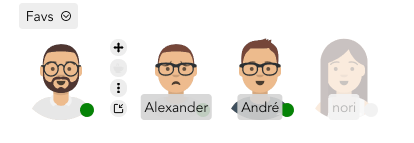
\includegraphics[width=0.5\textwidth]{./images/AT_hover.png}
    \caption{Ambient window while hovering over it }
\end{figure}


\medskip\noindent\textbf{People-centric} \\


\medskip\noindent\textbf{Workplace awareness} \\
Presence awareness is crucial and well-established in CSCW. Further, certain sources of potential interruptions are blocked inside AT if status is set to "Focus".

When fostering communication, it becomes important to not foster such communication in inopportune moments. Since concepts like presence/availability awareness, yet another part of informal awareness, are useful in reducing the number of interruptions \autocite{mark2005no}, Ambient Teams allows users to communicate their availability/interruptibility.


**Raising Hands**
Other consequences of remote work are that software developers have difficulties getting help when working remotely and finding experts \autocite{herbsleb2003empirical, espinosa2007team}, which is a significant driver for team performance \autocite{faraj2000coordinating}.


Indicating an non-interruptive request that is not urgent.

\medskip\noindent\textbf{Informal communication} \\
**Status Messaging (Microblogging)**
Micro-blogging is another strategy that allowed software engineers to share activities and moods with other team members with the result of feeling more connected to each other \autocite{dullemond2013fixing}.

Microblogging can help in feeling connected. Further, topics that are usually blogged about are informal [ehrlich2010microblogging](https://www.notion.so/ehrlich2010microblogging-2e87772b8033477e83c578385e4584e4)

"It [microblogging] is like a virtual coffee machine as a meeting place." [ebner2008microblogging](https://www.notion.so/ebner2008microblogging-d54afbbdd79240b7bac7e68609090385)

**Mood sharing**

Emotions are an important part of communication and can get lost/misunderstood inside text messages. [hook2008interactional](https://www.notion.so/hook2008interactional-0c875a7b714947ccb75cdd0856d5a366) enriched messages with colors indicating emotions and found it very useful.

"Furthermore, mood sharing and mood awareness appear to be good springboards for conversations and increased communication among users." [church2010study](https://www.notion.so/church2010study-050edec74b9840e887e2849ffd72cd51)

**Breakroom**

Our attempt to mimicking the water-cooler in the office. While awareness is critical, initiating a communication also has to be as easy as possible \autocite{chang2007out}.



\medskip\noindent\textbf{Main Window}


\medskip\noindent\textbf{Ambient Window}


\section{Preliminary Evaluation}
To evaluate the above mentioned research questions, a small pilot study will be conducted. The studyscope for this Master Thesis is to (1) develop a good study design that could then be used for a moreelaborate study in the future and (2) test it on a small scale.The preliminary evaluation will collect input on the the study design and capture preliminary feed-back on the efficacy and usefulness of the approach. The aim is to run the preliminary evaluation with5-10 participants (ideally all being part of 1-3 teams) and will be obtained with a post-study question-naire which contains both open- and close-ended questions to gather as much insights as possible. Inaddition to the qualitative data, participants’ activities and use of Ambient Teams will be logged toprovide insights into how they interacted with the app and which features they used the most.